\chapter{Introduction}

\textbf{Note}: All project files can be found at \url{https://www.github.com/okayjustin/roborodentia2017} \

\section{Definitions and Assumptions}
The robot is designed to only travel within a rectangular closed area of eight feet in the x direction and five feet in the y direction. The coordinate system is chosen as Cartesian with the origin placed at the bottom-left corner of the field. The position of the robot is always in the xy-plane since it cannot move vertically (z = 0). Therefore, $x$ refers to the robot position along the x-axis and ranges from 0 to 8 feet, and $y$ refers to position along the y-axis and ranges from 0 to 5 feet. Additionally, the robot can only rotate around the z-axis so $\theta$ refers to the angle of the robot in the xy-plane. Maintaining standard Cartesian coordinates, $\theta=\ang{0}$ is along the positive x direction while $\theta=\ang{90}$ is along the positive y direction.

\section{Cal Poly Roborodentia}
The robot is designed to compete in the 2018 Cal Poly Roborodentia, the university's annual intramural robotics competition, and thus conforms to its particular specifications and requirements. Briefly, autonomous robots collect and fire Nerf Rival Balls into nets to win points. A drawing of the field is shown below in Figure  \ref{fig:roborodentia_field}. 

\begin{figure}[H]   % [h] means here
	\centering
	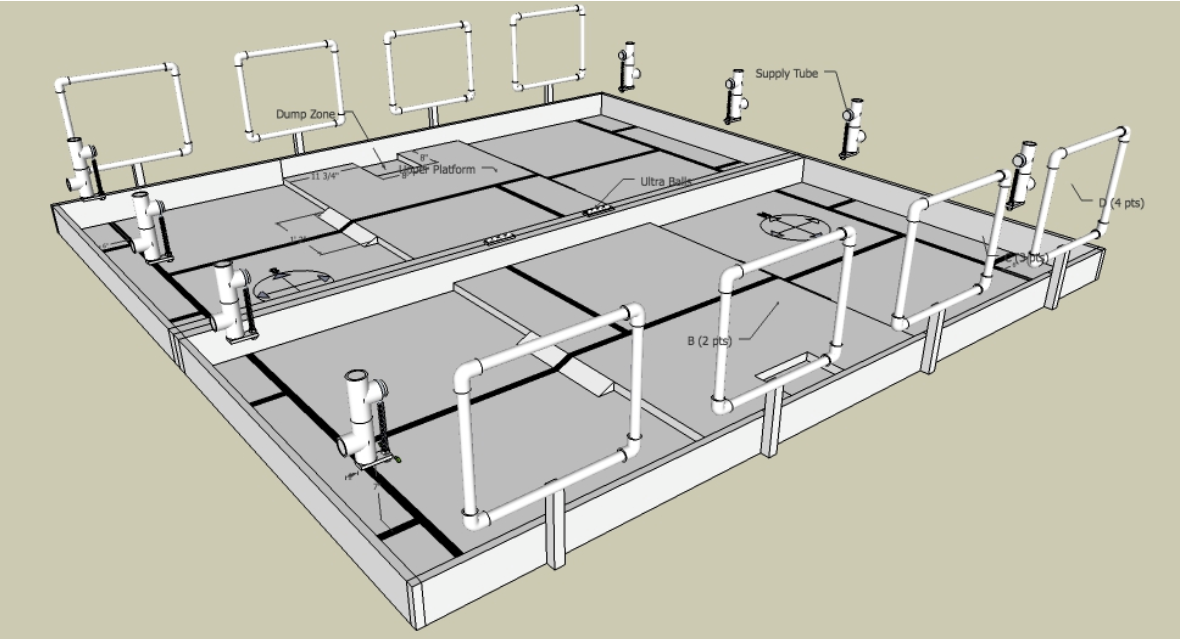
\includegraphics[width=7in]{figures/roborodentia_field.png}
	\caption{Roborodentia Field}
	\label{fig:roborodentia_field}
\end{figure}



